%GiG
\documentclass{beamer} 
\usetheme{Copenhagen}
\setbeamertemplate{navigation symbols}{}
\setbeamertemplate{headline}{}
\DeclareMathOperator*{\argmax}{arg\,max}

\usepackage{hyperref}


\definecolor{azure}{rgb}{0.0, 0.5, 1.0}
%\newcommand{\tblue}[1]{\textcolor{blue}{#1}}
\newcommand{\tblue}[1]{{\Large {\textcolor{azure}{#1}}}}
\newcommand{\thblue}[1]{{\Huge {\textcolor{azure}{#1}}}}
\newcommand{\hred}[1]{{\textcolor{red}{#1}}}
\newcommand{\furl}[1]{{\footnote{\url{#1}}}}

\title[Saravanan Thirumuruganathan] 
{Lecture 8: Dictionaries and Hash Tables}

\author[CSE 5311] 
{Instructor: Saravanan Thirumuruganathan}

\date[] 

\begin{document}

\begin{frame}
  \titlepage
\end{frame}

%\begin{frame}{Outline}
%  \tableofcontents
%  % You might wish to add the option [pausesections]
%\end{frame}

\section{Outline}

\begin{frame}
\frametitle {Outline}
\begin{enumerate}
\item Dictionaries
\item Hashing
\item Hash Tables
\item Briefly, DHTs and Bloom filters
\end{enumerate}
\end{frame}

\begin{frame}{In-Class Quizzes}
\begin{itemize}
\item {\Large {\bf URL:}} {\LARGE \bf \url{http://m.socrative.com/}} 
\item {\Large {\bf Room Name:} {\LARGE \bf 4f2bb99e}}
\end{itemize}
\end{frame}

\section{Dictionaries}

\begin{frame}{Dictionary ADT}
    \begin{itemize}
        \item Stores key-value pairs
        \item Required Operations:
        \begin{itemize}
            \item Insert
            \item Search (Membership check)
            \item Delete
        \end{itemize}
    \end{itemize}
\end{frame}

\begin{frame}{Motivation - I}

    \tblue{Caller ID Implementation:} 
    \begin{itemize}
        \item {\bf Objective:} Given phone number, output Caller's name
        \item Assume we need to worry about callers from Arlington only 
        \item What is the universe/input space? \pause
        \begin{itemize}
            \item Ignore first three digits (why?)
            \item Last 7 digits can input numbers between $0$ to $10^7-1$ 
            \item Number of phone numbers in Arlington way less than $10^7-1$
        \end{itemize}
    \end{itemize}
\end{frame}

\begin{frame}{Motivation - II}

    \tblue{Student ID Lookup:} 
    \begin{itemize}
        \item {\bf Objective:} Given student id, retrieve student information 
        \item Example: UTA graduate school, TA of this course
        \item What is the universe/input space? \pause
        \begin{itemize}
            \item Ignore four digits (why?)
            \item Last 6 digits can input numbers between $0$ to $10^6-1$ 
            \item Number of students in UTA/5311 is way less than $10^6$
        \end{itemize}
    \end{itemize}
\end{frame}


\begin{frame}{Potential Implementations}

    {\bf Possible Candidates:} \pause
    \begin{itemize}
        \item Linked List based
        \item Array based 
        \item Balanced trees
    \end{itemize}
\end{frame}

\begin{frame}{Space Vs Time Tradeoff}
    \begin{itemize}
        \item All our previous implementations optimized for time given linear storage cost
        \item What if time is more important than space?
        \item Think of companies like Google, Facebook, Amazon, AT\&T etc
    \end{itemize}
\end{frame}

\begin{frame}{Direct Address Tables\footnote{CLRS Fig 11.1}}
    \begin{center}
        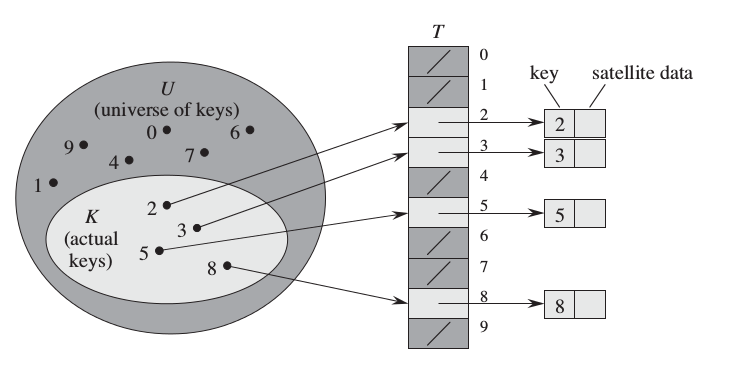
\includegraphics[scale=0.4]{directAddrssTable.png}
    \end{center}
\end{frame}

\begin{frame}[fragile]{Direct Address Tables}
    \begin{verbatim}
        DAT-Search(T,k):
            return T[k]

        DAT-Insert(T,x):
            T[x.key] = x

        DAT-Delete(T,x):
            T[x.key] = NULL
    \end{verbatim}
\end{frame}

\begin{frame}{Direct Address Tables}
    \begin{itemize}
        \item Represent input in an array 
        \item Each position/slot corresponds to a key in universe $U$
        \item Works well when $U$ is small
        \item Pro: \pause Fast
        \item Con: \pause Lot of space is wasted
    \end{itemize}
\end{frame}

\begin{frame}{Ideas to Improve DAT}
    \begin{itemize}
        \item Let size of universe be $N$
        \item Let Space budget be $m$ (for eg, $c \cdot \#\max$ elements)\pause
        \item Let \# elements inserted be $n$ 
        \item Caller ID Eg: $10^7-1$ vs $400K$ (size of Arlington)
        \item Student ID Eg: $10^6$ Vs $8000$ 
        \item 5311 Eg: $10^6$ vs $50$ \pause
        \item {\bf Insight:} Try to have space proportional to $m$ instead of $N$
    \end{itemize}
\end{frame}


\section{Hash Tables}

\begin{frame}{Hash Tables}
    \begin{center}
        \thblue{Hash Tables}
    \end{center}
\end{frame}

\begin{frame}{Hash Functions}
    \begin{itemize}
        \item {\bf Hash Function $h$:} Compute an array index from key value
        \item {\bf Input:} $1 .. N$
        \item {\bf Output:} $0 .. m-1$ 
        \item Formally, $h : U \rightarrow \{0, 1, \ldots, m-1\}$
        \item {\bf Requirement:} (Ideal): Uniformly scramble elements across array
        \begin{itemize}
            \item Efficient to compute (so peeking into array)
            \item Each array position is uniformly likely
        \end{itemize}
    \end{itemize}
\end{frame}

\begin{frame}{Hash Table\footnote{CLRS Fig 11.2}}
    \begin{center}
        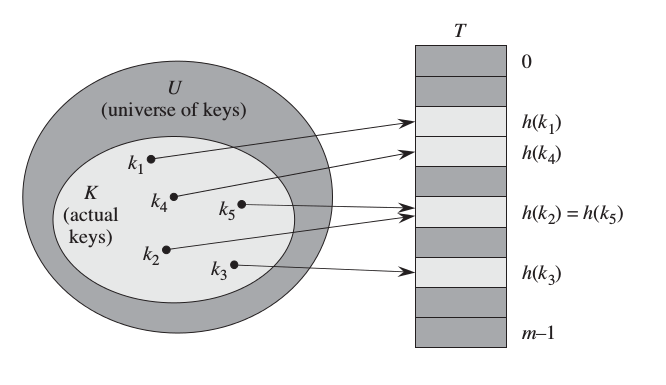
\includegraphics[scale=0.5]{hashTableAbstract.png}
    \end{center}
\end{frame}

\begin{frame}{Hash Function Design: Student ID Example}
    \begin{itemize}
        \item Space budget is $m=100$ (array with $100$ slots) 
        \begin{itemize}
            \item Objective: Design hash function $h(student\ id) \in \{0, 1, \ldots, 99\}$ \pause
            \item Last two digits of Student ID
            \item Student ID be $h(1000-000-188) \Rightarrow 88$ 
            \item Any two students with last two digits $88$?
        \end{itemize} 
        \item Space budget is $m=1000$ (array with $1000$ slots) \pause
        \begin{itemize}
            \item Objective: Design function $h(student\ id) \in \{0, 1, \ldots, 999\}$ \pause
            \item Last three digits of Student ID
            \item Student ID be $h(1000-000-188) \Rightarrow 188$ 
            \item Any two students with last two digits $188$?
        \end{itemize} 
        \item Tradeoff between Space and Collisions
    \end{itemize}
\end{frame}

\begin{frame}{Good and Bad Hash Functions}
    \begin{itemize}
        \item 10-digit phone numbers
        \begin{itemize}
            \item First three digits: \pause Bad! (why?)
            \item Last three digits: \pause Better (why?)
        \end{itemize} 
        \item 10-digit UTA student id 
        \begin{itemize}
            \item First three digits: Bad! (why?)
            \item Last three digits: Better (why?)
        \end{itemize} 
        \item 9-digit SSN
        \begin{itemize}
            \item First three digits: \pause Bad! (why?)
            \item Last three digits: \pause Better (why?)
        \end{itemize} 
    \end{itemize}
\end{frame}

\begin{frame}{Hash Function Design}
    \begin{itemize}
        \item {\bf Division/Modular:} $h(k) = k \mod m$  
        \begin{itemize}
            \item Alternative: Mod by a prime $P$
            \item Java Strings: $P=31$
        \end{itemize} 
        \item {\bf Multiplication:} $h(k) = \lfloor m(kA \mod 1) \rfloor$  
        \begin{itemize}
            \item $0 < A < 1$
            \item Take the fractional part and multiply it by $m$
        \end{itemize} 
        \item Universal hashing
    \end{itemize}
\end{frame}

\subsection{Collisions}
\begin{frame}{Collisions}
    \begin{itemize}
        \item When two items are hashed to same slot $h(k_i) = h(k_j)$
        \item Collision Resolution Techniques
        \begin{itemize}
            \item Separate Chaining
            \item Open Addressing: Linear probing, Quadratic probing, Double Hashing
        \end{itemize}
    \end{itemize}
\end{frame}


\begin{frame}{Separate Chaining\footnote{CLRS Fig 11.3}}
    \begin{itemize}
        \item Idea: Place all elements that hash to same slot in a linked list 
    \end{itemize}
    \begin{center}
        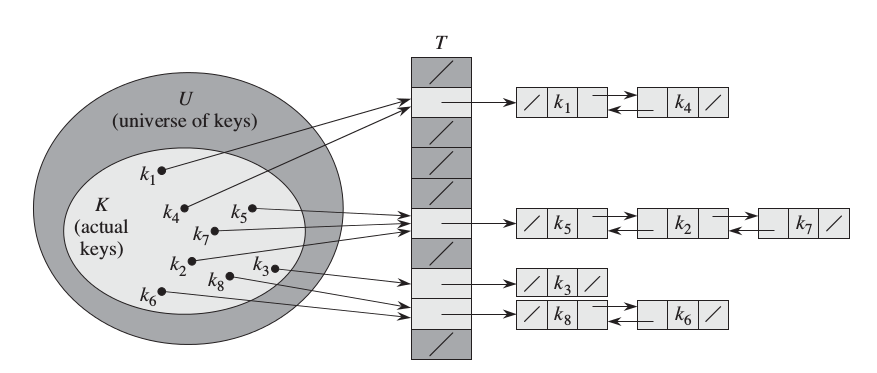
\includegraphics[scale=0.36]{hashTablesChaining.png}
    \end{center}
\end{frame}

\begin{frame}[fragile]{Separate Chaining}
    \begin{verbatim}
Chained-Hash-Insert(T,x):
    Insert x at head of linked list T[h(x.key)]

Chained-Hash-Search(T,k):
    Search for element with key k in T[h(k)]

Chained-Hash-Delete(T,x):
    Delete x from linked list T[h(x.key)] 
    \end{verbatim}
\end{frame}

\begin{frame}{Open Addressing}
    \begin{itemize}
        \item Separate Chaining used an external data structure to store all elements that collide
        \item Open Addressing 
        \begin{itemize}
            \item Do not use external storage (one element per slot)
            \item Use hash table itself to store elements that collide
            \item When a new key collides, find an empty slot and put it there
        \end{itemize}
        \item Handling deletions is very messy - we will not discuss it here
    \end{itemize}
\end{frame}

\begin{frame}{Linear Probing}

    {\bf Linear Probing:}
    \begin{itemize}
        \item Using hash function, map key to an array index (say $i$)
        \item Put element at slot $i$ if it is free
        \item If not try $i+1$, $i+2$, etc
        \item Roll around to start if needed
    \end{itemize}
\end{frame}

\begin{frame}{Linear Probing: Example\footnote{\url{https://ece.uwaterloo.ca/~cmoreno/ece250/2012-01-30--hash_tables.pdf}}}
    \begin{itemize}
        \item Objective: Insert elements $\langle 81, 70, 97, 60, 51, 38, 89, 68, 24 \rangle$ 
        \item Resolve collisions via linear probing 
        \item Hash function $h(k) = k \% 10$ (i.e. take last digit)
    \end{itemize}
    \begin{center}
        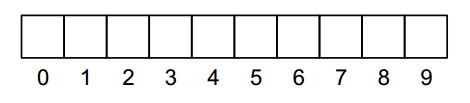
\includegraphics[scale=0.5]{linearProbing1.png}
    \end{center}
\end{frame}

\begin{frame}{Linear Probing: Example\footnote{\url{https://ece.uwaterloo.ca/~cmoreno/ece250/2012-01-30--hash_tables.pdf}}}
    \begin{itemize}
        \item Objective: Insert elements $\langle \textcolor{red}{81, 70, 97}, 60, 51, 38, 89, 68, 24 \rangle$ 
        \begin{center}
            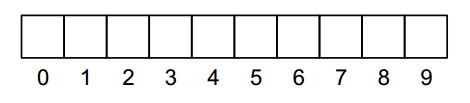
\includegraphics[scale=0.5]{linearProbing1.png}
        \end{center}
        \item First three elements have no collisions \pause
        \begin{center}
            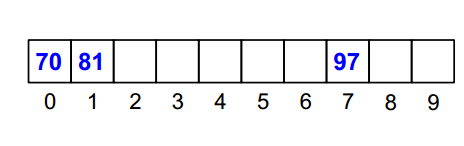
\includegraphics[scale=0.5]{linearProbing2.png}
        \end{center}
    \end{itemize}
\end{frame}

\begin{frame}{Linear Probing: Example\footnote{\url{https://ece.uwaterloo.ca/~cmoreno/ece250/2012-01-30--hash_tables.pdf}}}
    \begin{itemize}
        \item Objective: Insert elements $\langle 81, 70, 97, \textcolor{red}{60}, 51, 38, 89, 68, 24 \rangle$ 
        \item Collision when inserting $60$ 
        \begin{center}
            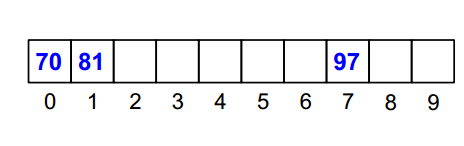
\includegraphics[scale=0.5]{linearProbing2.png} \pause
        \end{center}
        \item Check slot 1 - it is full
        \item Check slot 2 - it is empty, so insert it
        \begin{center}
            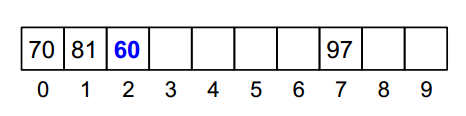
\includegraphics[scale=0.5]{linearProbing3.png}
        \end{center}
    \end{itemize}
\end{frame}

\begin{frame}{Linear Probing: Example\footnote{\url{https://ece.uwaterloo.ca/~cmoreno/ece250/2012-01-30--hash_tables.pdf}}}
    \begin{itemize}
        \item Objective: Insert elements $\langle 81, 70, 97, 60, \textcolor{red}{51}, 38, 89, 68, 24 \rangle$ 
        \item Collision when inserting $51$ 
        \begin{center}
            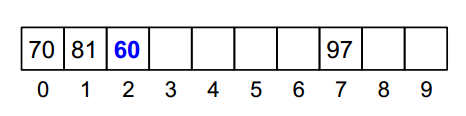
\includegraphics[scale=0.5]{linearProbing3.png} \pause
        \end{center}
        \item Check slot 2 - it is full
        \item Check slot 3 - it is empty, so insert it
        \begin{center}
            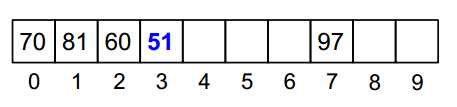
\includegraphics[scale=0.5]{linearProbing4.png}
        \end{center}
    \end{itemize}
\end{frame}

\begin{frame}{Linear Probing: Example\footnote{\url{https://ece.uwaterloo.ca/~cmoreno/ece250/2012-01-30--hash_tables.pdf}}}
    \begin{itemize}
        \item Objective: Insert elements $\langle 81, 70, 97, 60, 51, \textcolor{red}{38, 89}, 68, 24 \rangle$ 
        \item No collisions when inserting $38$ and $89$
        \begin{center}
            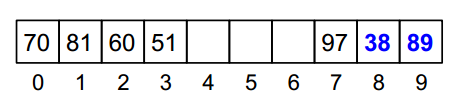
\includegraphics[scale=0.5]{linearProbing5.png} 
        \end{center}
    \end{itemize}
\end{frame}


\begin{frame}{Linear Probing: Example\footnote{\url{https://ece.uwaterloo.ca/~cmoreno/ece250/2012-01-30--hash_tables.pdf}}}
    \begin{itemize}
        \item Objective: Insert elements $\langle 81, 70, 97, 60, 51, 38, 89, \textcolor{red}{68}, 24 \rangle$ 
        \item Collision when inserting $68$ 
        \begin{center}
            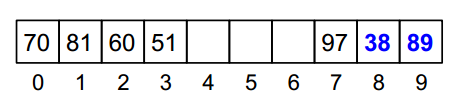
\includegraphics[scale=0.5]{linearProbing5.png} \pause
        \end{center}
        \item Check slot $9$ - it is full \pause
        \item Wrap around: Check slots $0, 1, 2, 3$
        \item Insert $68$ in slot $4$
        \begin{center}
            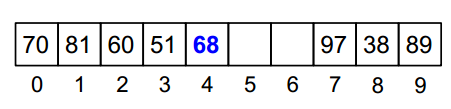
\includegraphics[scale=0.5]{linearProbing6.png}
        \end{center}
    \end{itemize}
\end{frame}


\begin{frame}{Linear Probing: Example\footnote{\url{https://ece.uwaterloo.ca/~cmoreno/ece250/2012-01-30--hash_tables.pdf}}}
    \begin{itemize}
        \item Objective: Insert elements $\langle 81, 70, 97, 60, 51, 38, 89, 68, \textcolor{red}{24} \rangle$ 
        \item Collision when inserting $68$ 
        \begin{center}
            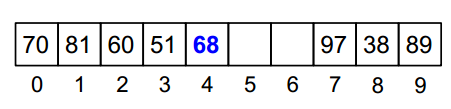
\includegraphics[scale=0.5]{linearProbing6.png} \pause
        \end{center}
        \item Check slot $4$ - it is full \pause
        \item Insert $24$ in slot $5$
        \begin{center}
            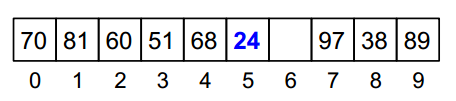
\includegraphics[scale=0.5]{linearProbing7.png}
        \end{center}
    \end{itemize}
\end{frame}


\begin{frame}{Linear Probing: Example\footnote{\url{https://ece.uwaterloo.ca/~cmoreno/ece250/2012-01-30--hash_tables.pdf}}}
        
       {\bf Searching with Linear Probing:}
        \begin{center}
            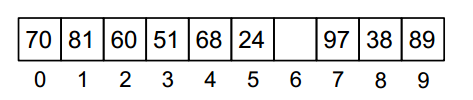
\includegraphics[scale=0.5]{linearProbing8.png} 
        \end{center}

    \begin{itemize}
        \item Easy Case: Search($T, 81$) 
        \item Harder Case I: Search($T, 60$) 
        \item Harder Case II: Search($T, 68$) 
        \item Harder Case III: Search($T, 80$)
    \end{itemize}
\end{frame}

\begin{frame}{Linear Probing Issues: Primary Clustering\footnote{\url{https://ece.uwaterloo.ca/~cmoreno/ece250/2012-01-30--hash_tables.pdf}}}
    \begin{itemize}
        \item Remember the scenario of inserting $68$
        \begin{center}
            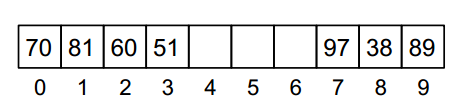
\includegraphics[scale=0.5]{linearProbingClustering.png} 
        \end{center} 
        \item Had to travel long to find next empty slot
        \item Once collision happens, new keys are more likely to hash in middle of blocks 
        \item So you have to spend more time to find an empty slot (extending the block size)
        \item You now increased the chance of a collision in the block!
    \end{itemize}
\end{frame}

\begin{frame}{Fixing Primary Clustering}
    \begin{itemize}
        \item Idea: Look for empty slots increasingly further away from original slot
        \item Probe Sequence: The order in which successive slots are checked
        \item Linear Probing: $h(k,i) = h'(k) + i$
        \item Probe sequence for Linear Probing: $$h'(k), h'(k)+1, h'(k)+2, \ldots$$
    \end{itemize}
\end{frame}

\begin{frame}{Fixing Primary Clustering}
    \begin{itemize}
        \item Probe sequence for LP: $h'(k), h'(k)+1, h'(k)+2, \ldots$
        \item Quadratic probing:  $h(k,i) = h'(k) + c_1 i + c_2 i^2$
            \begin{itemize}
                \item Probe sequence when $c_1=0, c_2=1$,\\ 
                    \qquad $h'(k), h'(k)+\textcolor{red}{1^2}, h'(k)+\textcolor{red}{2^2}, \ldots$
            \end{itemize}
        \item Double Hashing
            \begin{itemize}
                \item Choose two hash functions $h_1$ and $h_2$
                \item Use $h_1$ first
                \item If no collision, all is well
                \item Else use the probing sequence \\ \qquad $h(k,i) = ( h_1(k) + i \cdot h_2(k)) \mod m$
            \end{itemize}
        \item Search: Follow same procedure till you find the element or an empty slot 
    \end{itemize}
\end{frame}

\begin{frame}{Hash Tables: Practical Advice I}
    \begin{itemize}
        \item Load factor $\alpha = n/m$ (\#elements / \#table size)
        \item Low $\alpha$: wasted space 
        \item High $\alpha$: long time for insert and search
        \item If you know $n$, pass it to Hash table (e.g. Java, Python)
        \item The data structure will be much faster
        \item For eg, most languages will set $m = \frac{4}{3} n$ (with $\alpha = \frac{3}{4}$)
        \item {\bf Re-hashing:} Automatically adjusting number of budgets
        \item If $\alpha$ becomes too low or high, {\bf re-hashing} happens (it is bad!)
    \end{itemize}
\end{frame}

\begin{frame}{Hash Tables: Practical Advice II}
    \begin{itemize}
        \item Load factor $\alpha = n/m$ (\#elements / \#table size)
        \item Chaining can be used when $\alpha < ~0.9$
        \item Linear probing is used when table is sparse ($\alpha ~ 0.5$)
        \item Double hashing is used when $\alpha < 0.66$
        \item With {\bf good} hash functions, Hash table outperforms BST, RBT etc
        \item Double hashing: $h_2(k)$ can never be $0$ (else you get infinite loop)
    \end{itemize}
\end{frame}



\section{DHTs}
\begin{frame}{}
    \begin{center}
        \thblue{Distributed Hash Tables (DHTs)}
    \end{center}
\end{frame}

\begin{frame}{Distributed Hash Tables (DHTs)}
    \begin{itemize}
        \item {\bf Idea:} Distribute the hash table content across many machines (typically a P2P network) 
        \item {\bf Motivation:}
        \begin{itemize}
            \item Scalability: Eg. CDNs, NoSQL DBs
            \item Fault Tolerance: Eg. Robust data archiving 
            \item Decentralization: Eg. BitTorrent
        \end{itemize}
        \item {\bf Issue:} We now have to determine which node to store data too!
    \end{itemize}
\end{frame}

\begin{frame}{Distributed Hash Tables (DHTs)}
    
    {\bf Applications:}
    \begin{itemize}
        \item Any internet scale application would have to use DHT
        \item Domain Name Service (hierarchical)
        \item File Sharing and Caching
        \item Archival/Retrieval of content (Eg. Dropbox: Deduplication)
        \item BitTorrent and other {\bf trackerless} sharing sites
        \item Load balancing
        \item Anonymous web browsing 
        \item Serverless email systems
    \end{itemize}
\end{frame}

\begin{frame}{DHTs: Visualization\footnote{\url{http://www.cs.princeton.edu/courses/archive/spr09/cos461/docs/lec18-dhts.pdf}}}

    \begin{center}
        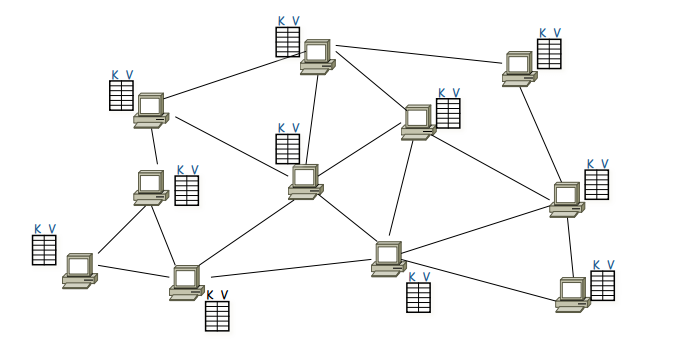
\includegraphics[scale=0.4]{dhtViz.png}
    \end{center}
\end{frame}

\begin{frame}{DHTs: Put\footnote{\url{http://www.cs.princeton.edu/courses/archive/spr09/cos461/docs/lec18-dhts.pdf}}}

    \begin{center}
        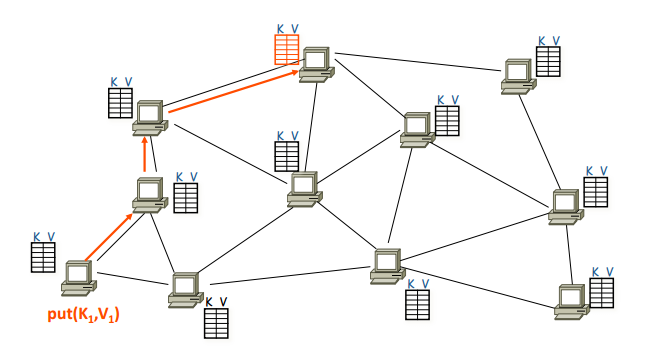
\includegraphics[scale=0.4]{dhtPut.png}
    \end{center}
\end{frame}

\begin{frame}{DHTs: Get\footnote{\url{http://www.cs.princeton.edu/courses/archive/spr09/cos461/docs/lec18-dhts.pdf}}}

    \begin{center}
        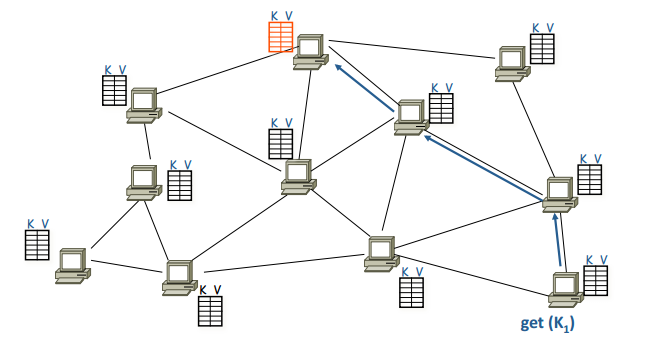
\includegraphics[scale=0.4]{dhtGet.png}
    \end{center}
\end{frame}


\begin{frame}{DHTs: Sample Implementation\footnote{\url{http://www.ietf.org/old/2009/proceedings/06mar/slides/plenaryt-2.pdf}}}

    {\bf Chord Ring:} Routing, Joining, Replication
    \begin{center}
        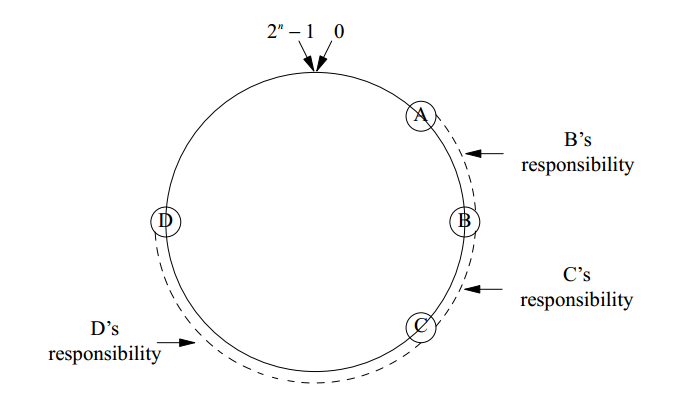
\includegraphics[scale=0.4]{chordRing.png}
    \end{center}
\end{frame}

\begin{frame}{DHTs: Consistent Hashing}
    \begin{itemize}
        \item Consistent Hashing function: Special type of hashing function
        \item When $m$ (\#slots) or $n$ (\#item) is changed,  at most $O(\lg n)$ items have to be moved
        \item Great idea for P2P systems with node arrival and removal
    \end{itemize}
\end{frame}

\section{Bloom Filters}
\begin{frame}{}
    \begin{itemize}
        \item GiG
    \end{itemize}
\end{frame}

\begin{frame}{}
    \begin{center}
        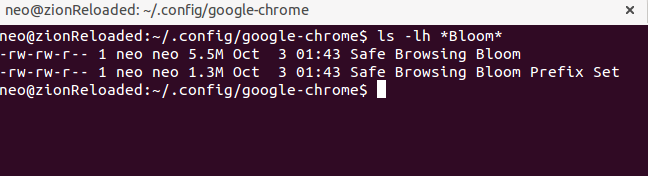
\includegraphics[scale=0.5]{bloomFilterGoogleChrome.png}
    \end{center}
\end{frame}

\begin{frame}{}
    \begin{itemize}
        \item GiG
    \end{itemize}
\end{frame}

\begin{frame}{}
    \begin{itemize}
        \item GiG
    \end{itemize}
\end{frame}

\begin{frame}{}
    \begin{itemize}
        \item GiG
    \end{itemize}
\end{frame}

\begin{frame}{}
    \begin{itemize}
        \item GiG
    \end{itemize}
\end{frame}

\begin{frame}{}
    \begin{itemize}
        \item GiG
    \end{itemize}
\end{frame}

\begin{frame}{}
    \begin{itemize}
        \item GiG
    \end{itemize}
\end{frame}



\section{Summary}

\begin{frame}{Summary}

\tblue{Major Concepts:}
\begin{itemize}
\item Dictionary ADT 
\item Hash Tables  
\item Hashing, Collision Resolution
\item DHTs, Bloom Filters
\end{itemize}
\end{frame}


\end{document}

